\begin{landscape}
\chapter{State Machine Overview}
\label{cha:state-mach-overv}

\begin{figure}[h]
  \centering
  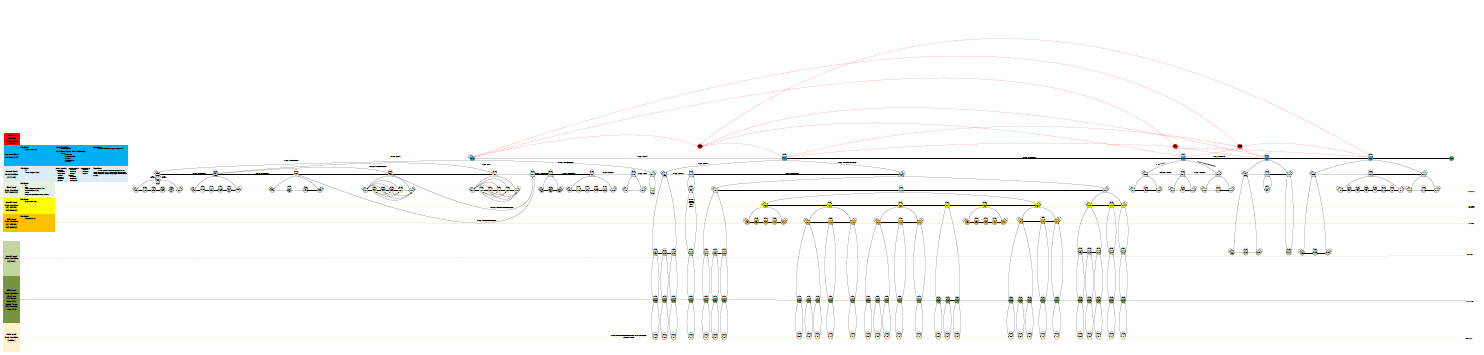
\includegraphics[width=1\linewidth]{appendix1.PNG}
\end{figure}
NOTE: A digital copy is available on the Syracuse University Google\textregistered
Drive in both pdf and visio formats. The visio formatted document contains
comments with descriptions, possible HOL implementation, and references
to the Ranger Handbook (where applicable).

\chapter{PB UML Class Diagram}
\label{cha:pb-uml-class}

\begin{figure}[h]
  \centering
  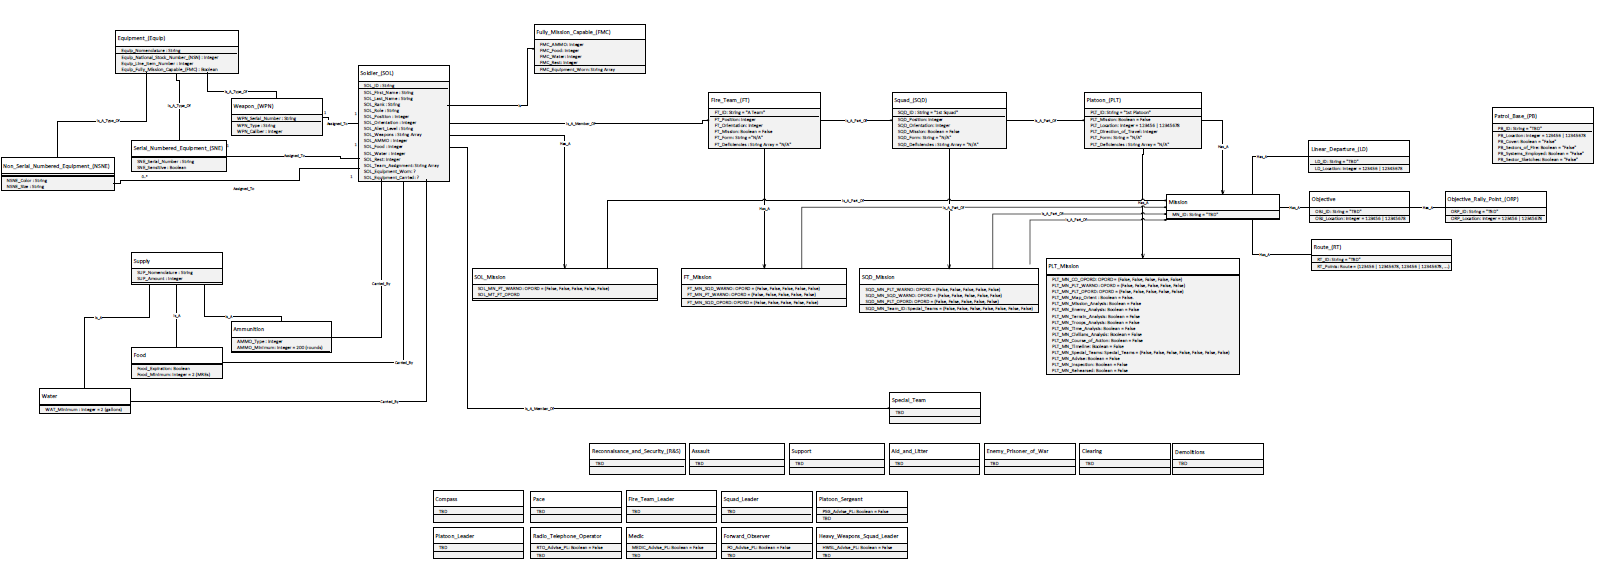
\includegraphics[width=1\linewidth]{appendix2.png}
\end{figure}
NOTE: A digital copy is available on the Syracuse University Google\textregistered
Drive in both pdf and visio formats. The visio formatted document contains
comments with descriptions, possible HOL implementation, and references
to the Ranger Handbook (where applicable).



\chapter{PLAN_PB DFD Level 0}
\label{cha:planpb-dfd-level-2}

\begin{figure}[h]
  \centering
  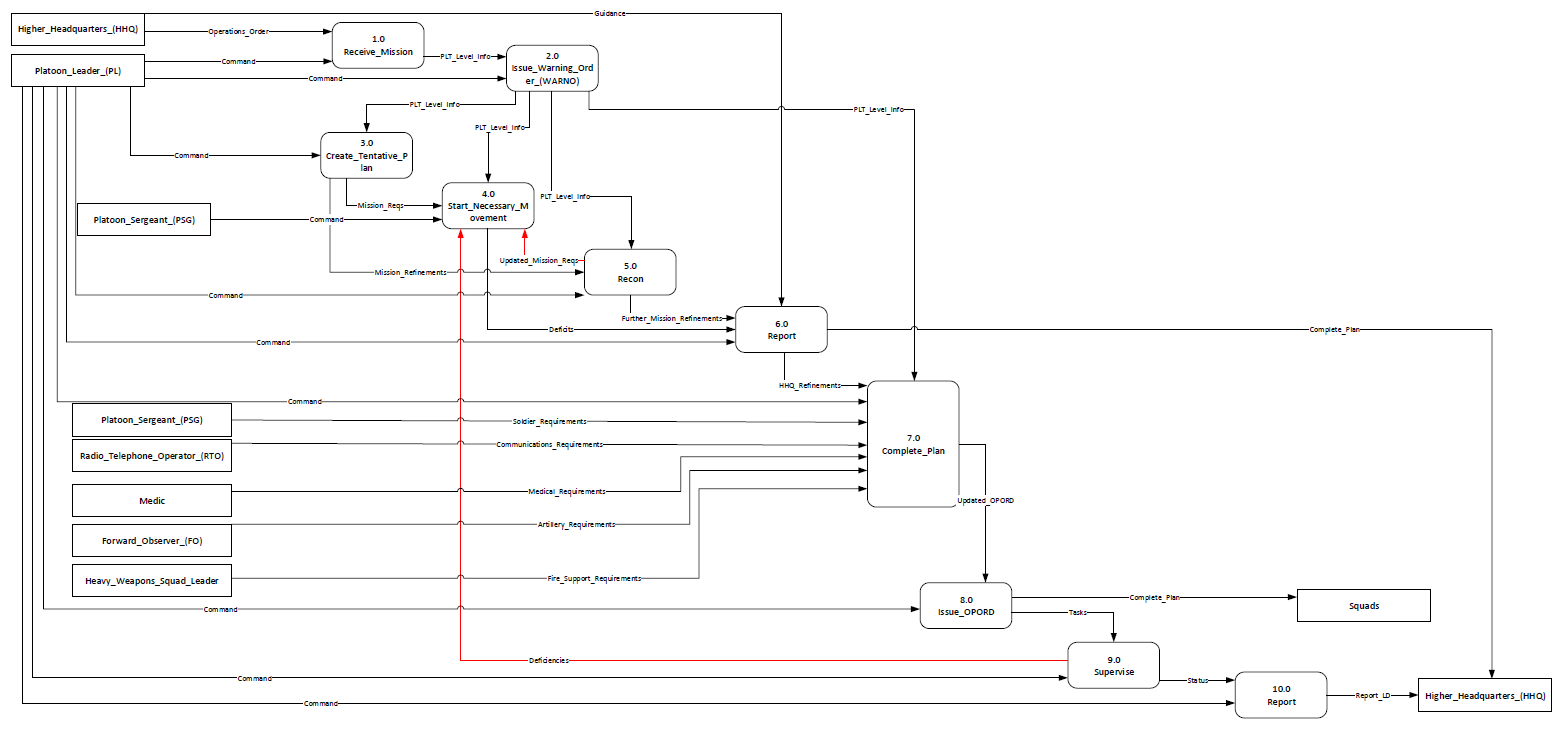
\includegraphics[width=1\linewidth]{appendix3.png}
\end{figure}
NOTE: A digital copy is available on the Syracuse University Google\textregistered
Drive in both pdf and visio formats. The visio formatted document contains
comments with descriptions, possible HOL implementation, and references
to the Ranger Handbook (where applicable).
\end{landscape}

% \chapter{Next State, Next Output Table}
% \label{cha:next-state-next}

% \begin{table}[h!]
% \begin{center}
%   \resizebox{\textwidth}{!}{\begin{tabular}{|m{5em}|c|m{8em}|m{9em}|m{8em}|m{8em}|m{8em}|m{9em}|}
%                               \hline
%     \multicolumn{8}{|c|}{ }\\
%     \multicolumn{8}{|c|}{\textcolor{cyan}{Next State}, Next Output Table}\\
%     \multicolumn{8}{|c|}{ }\\
%     \hline\hline
%     & \cellcolor{cyan}State &&&&&&\\
%     \hline
%      \rowcolor{lime}Commands/ input &  \cellcolor{white}next state, next output  & crossLD & conductORP & moveToPB & conductPB & completePB & incomeplete \\
%      \hline
%      & \cellcolor{cyan}PLAN_PB & \textcolor{cyan}{MOVE_TO_ORP}, MoveToORP & \rowcolor{lightgray}  &  &&& \cellcolor{white}\textcolor{cyan}{PLAN_PB}, PlanPB \\
%     \hline
%      & \cellcolor{cyan}MOVE_TO_ORP & \rowcolor{lightgray}& \cellcolor{white}\textcolor{cyan}{CONDUCT_ORP}, ConductORP & & & & \cellcolor{white}\textcolor{cyan}{MOVE_TO_ORP}, MoveToORP \\
%     \hline
%      & \cellcolor{cyan}CONDUCT_ORP &\rowcolor{lightgray} & & \cellcolor{white}\textcolor{cyan}{MOVE_TO_PB}, MoveToPB & & & \cellcolor{white}\textcolor{cyan}{CONDUCT_ORP}, ConductORP \\
%     \hline
%      &\cellcolor{cyan} MOVE_TO_PB & \rowcolor{lightgray}&&& \cellcolor{white}\textcolor{cyan}{CONDUCT_PB}, ConductPB && \cellcolor{white}\textcolor{cyan}{MOVE_TO_PB}, MoveToPB \\
%     \hline
%      & \cellcolor{cyan}CONDUCT_PB & \rowcolor{lightgray}&&&& \cellcolor{white}\textcolor{cyan}{COMPLETE_PB}, CompletePB & \cellcolor{white}\textcolor{cyan}{CONDUCT_PB}, ConductPB \\
%     \hline
%      & \cellcolor{cyan}COMPLETE_PB & \rowcolor{lightgray} &&&&& \\
%     \hline

%  \end{tabular}
%  }
% \end{center}
% \end{table}

\chapter{Source Code for OMNITypeScript.sml}
\label{cha:source-code-omnityp}
The following code if from \emph{OMNITypeScript.sml}
\lstinputlisting{../HOL/OMNITypeScript.sml}

\chapter{Source Code for satListScript.sml}
\label{cha:source-code-satl}
The following code is from \emph{satListScript.sml}
\lstinputlisting{../HOL/satListScript.sml}

\chapter{Source Code for ssm11Script.sml}
\label{cha:source-code-ssm11scr}
The following code is from \emph{ssm11Script.sml}
\lstinputlisting{../HOL/ssm11Script.sml}

\chapter{Source Code for ssmScript.sml}
\label{cha:source-code-ssmscr}
The following code is from \emph{ssmScript.sml}
\lstinputlisting{../HOL/ssmScript.sml}

\chapter{Source Code for ssminfRules.sml}
\label{cha:source-code-ssminfr}
The following code is from \emph{ssminfRules.sml}
\lstinputlisting{../HOL/ssminfRules.sml}

\chapter{Source Code for ssminfRules.sig}
\label{cha:source-code-ssminfr-1}
The following code is from \emph{ssminfRules.sml}
\lstinputlisting{../HOL/ssminfRules.sig}

\chapter{Source code for ssmPBScript.sml}
\label{cha:source-code-ssmpbscr}
The following code is from \emph{ssmPBScript.sml}
\lstinputlisting{../HOL/ssmPB/ssmPBScript.sml}

\chapter{Source Code for PBTypeScript.sml}
\label{cha:source-code-pbtyp}
The following code is from \emph{PBTypeScript.sml}
\lstinputlisting{../HOL/ssmPB/PBTypeScript.sml}

\chapter{Source Code for MoveToORPTypeScript.sml}
\label{cha:source-code-movet}
The following code is from \emph{MoveToORPTypeScript.sml}
\lstinputlisting{../HOL/ssmPB/subLevel/ssmMoveToORP/MoveToORPTypeScript.sml}

\chapter{Source Code for ssmMoveToORPScript.sml}
\label{cha:source-code-ssmm}
The following code is from \emph{ssmMoveToORPScript.sml}
\lstinputlisting{../HOL/ssmPB/subLevel/ssmMoveToORP/ssmMoveToORPScript.sml}

\chapter{Source Code for ConductORPTypeScript.sml}
\label{cha:source-code-cond}
The following code is from \emph{ConductORPTypeScript.sml}
\lstinputlisting{../HOL/ssmPB/subLevel/ssmConductORP/ConductORPTypeScript.sml}

\chapter{Source Code for ssmConductORPScript.sml}
\label{cha:source-code-ssmc}
The following code is from \emph{ssmConductORPScript.sml}
\lstinputlisting{../HOL/ssmPB/subLevel/ssmConductORP/ssmConductORPScript.sml}

\chapter{Source Code for MoveToPBTypeScript.sml}
\label{cha:source-code-movet-1}
The following code is from \emph{MoveToPBTypeScript.sml}
\lstinputlisting{../HOL/ssmPB/subLevel/ssmMoveToPB/MoveToPBTypeScript.sml}

\chapter{Source Code for ssmMoveToPBScript.sml}
\label{cha:source-code-ssmm-1}
The following code is from \emph{ssmMoveToPBScript.sml}
\lstinputlisting{../HOL/ssmPB/subLevel/ssmMoveToPB/ssmMoveToPBScript.sml}

\chapter{Source Code for ConductPBTypeScript.sml}
\label{cha:source-code-cond-1}
The following code is from \emph{ConductPBTypeScript.sml}
\lstinputlisting{../HOL/ssmPB/subLevel/ssmConductPB/ConductPBTypeScript.sml}

\chapter{Source Code for ssmConductPBScript.sml}
\label{cha:source-code-ssmc-1}
The following code is from \emph{ssmConductPBScript.sml}
\lstinputlisting{../HOL/ssmPB/subLevel/ssmConductPB/ssmConductPBScript.sml}

\chapter{OMNIReport.pdf}
\label{cha:omnireport.pdf}
The following is a copy of the \hypertarget{OMNIReport}{OMNIReport.pdf}.
%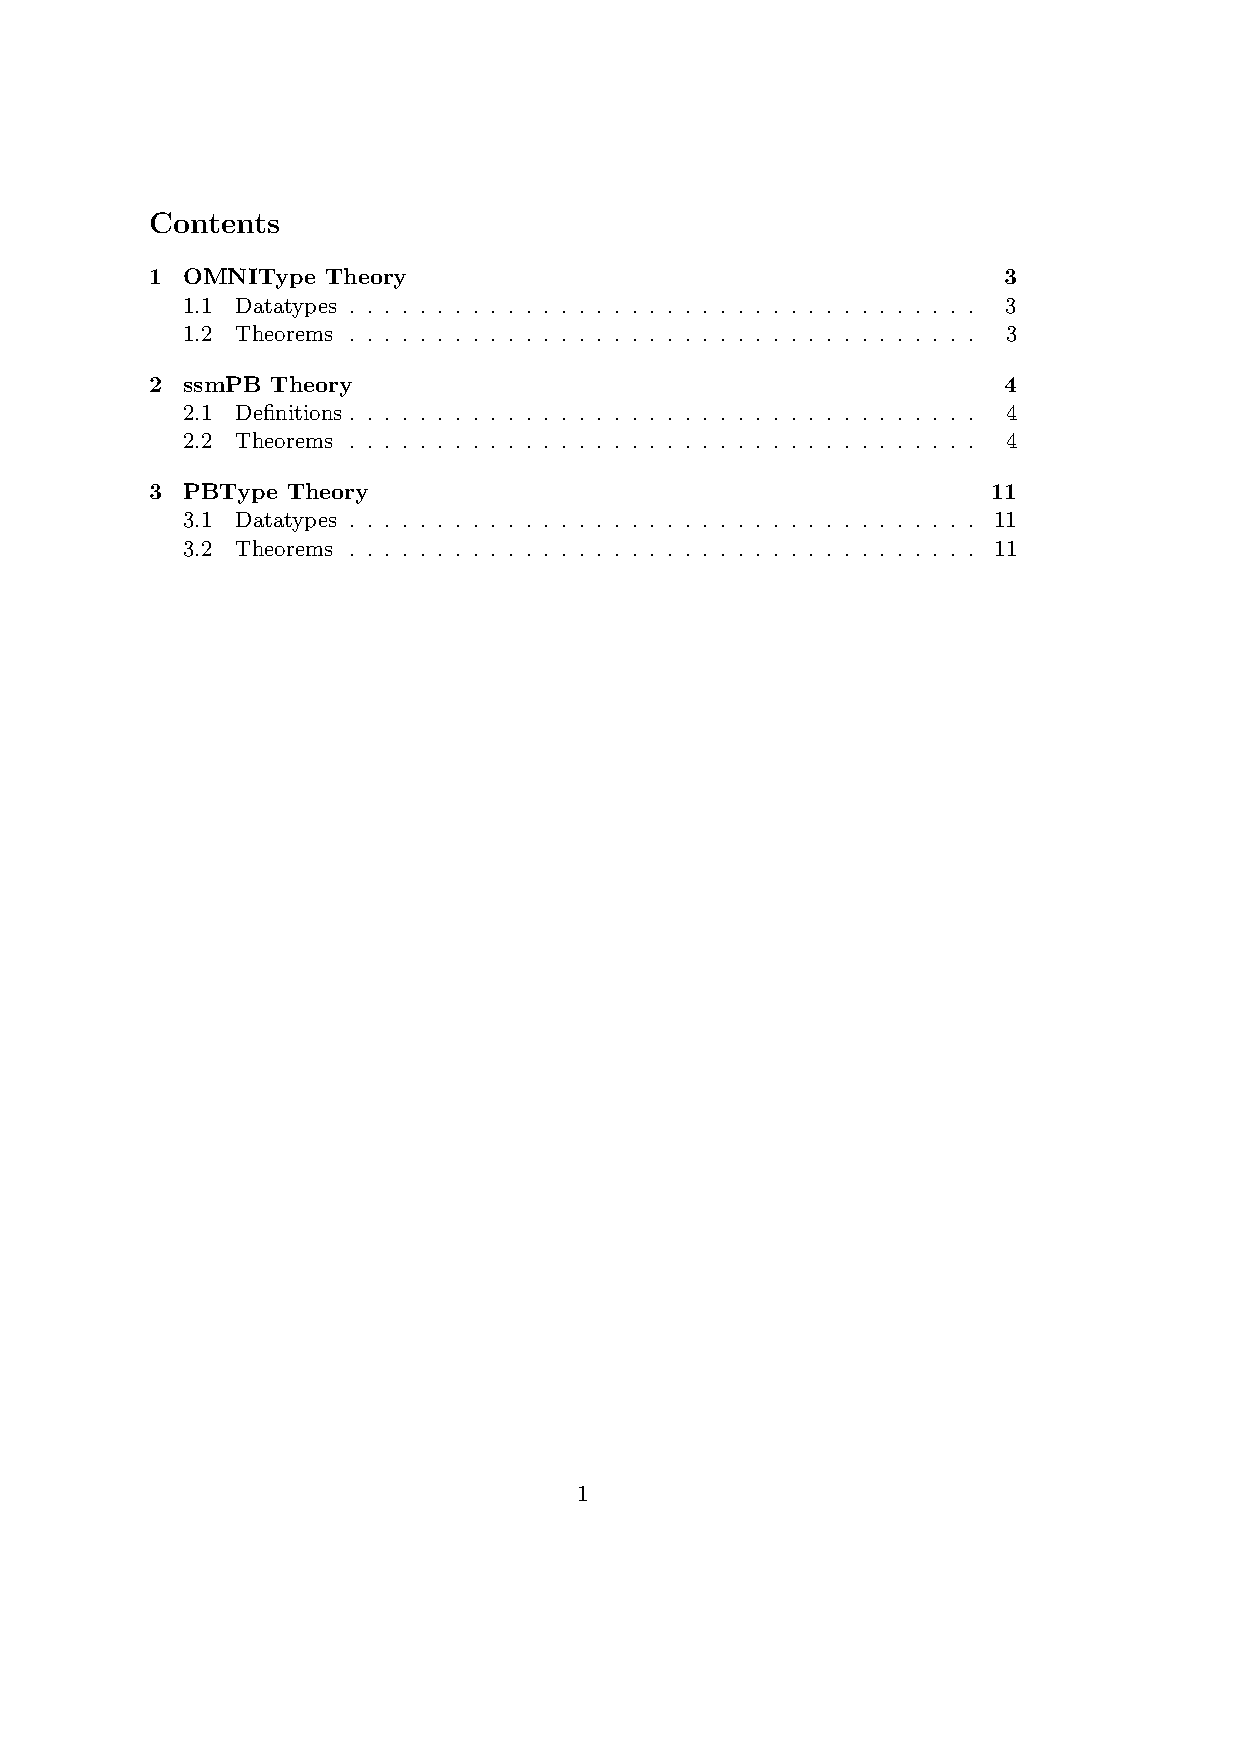
\includepdf[pages={1-}, scale = 1]{../HOL/HOLReportsOMNI/OMNIReport.pdf}

\chapter{Symbols, Abbreviations, and Acronyms}
\label{cha:symb-abbr-acronyms}

\begin{align*}
&DFD\;\;\;\;\;&Data Flow Diagram\ \\
&HHQ\;\;\;\;\;&Higher Headquarters\ \\ 
&HOL\;\;\;\;\;&High Order Logic\ \\
&LD\;\;\;\;\;&Line of Departure/Linear Departure\ \\
&NMC\;\;\;\;\;&Non-Mission Capable\ \\
&OPORD\;\;\;\;\;&Operation Order\ \\
&PB\;\;\;\;\;&Patrol Base\ \\
&PL\;\;\;\;\;&Platoon Leader\ \\
&PolyML\;\;\;\;\;&Poly Metalanguage\ \\
&PSG\;\;\;\;\;&Platoon Sergeant\ \\
&TLP\;\;\;\;\;&Troop Leading Procedure\ \\
&UML\;\;\;\;\;&Unified Modeling Language\ \\
\end{align*}

% ---- this points LaTeX to PatrolBaseDoc.tex ----
% Local Variables:
% TeX-master: "../PatrolBaseDoc"
% End: